% ====================================================================
%+
% SECTION:
%    MW_Disk.tex
%
% CHAPTER:
%    galaxy.tex
%
% ELEVATOR PITCH:
%
%-
% ====================================================================

\section{Populations in the Milky Way Disk}
\def\secname{MW_Disk}\label{sec:\secname}

\credit{willclarkson}, \credit{caprastro}, \credit{cbritt4}, \credit{chomiuk}

Many populations of great importance to Astronomy exist predominantly
in or near the Galactic Plane, and yet are sufficiently
sparsely-distributed (and/or faint enough) that LSST is likely to be
the only facility in the forseeable future that will be able to
identify a statistically meaningful sample. Some (such as the novae
that allow detailed study of the route to Type Ia Supernovae) offer
unique laboratories to study processes of fundamental importance to
astrophysics at all scales. Others (like intra-disk microlensing
events) offer the {\it only} probe of important populations.

%An important collateral benefit of studies in the plane with an
%LSST-like facility, is improved mapping of the distribution and
%observational effects of the ISM (particularly dust), which is of
%importance to all IR/Optical/UV observational studies. \new{Due to its
%  importance for {\it all} Milky Way Astronomy, a separate Section is
%  devoted to the impact of observing strategy on the utility of LSST
% data to constrain the distribution of interstellar dust in three
%  dimensions (\autoref{sec:MW_Dust}).}

% --------------------------------------------------------------------

\subsection{Target measurements and discoveries}
\label{sec:\secname:MW_Disk_targets}

%Describe the discoveries and measurements you want to make.

%Now, describe their response to the observing strategy. Qualitatively,
%how will the science project be affected by the observing schedule and
%conditions? In broad terms, how would we expect the observing strategy
%to be optimized for this science?

We have identified four science cases within the general area of Milky
Way Disk studies, that will have a diversity of dependencies on
observing strategy (e.g. slow intrinsic variability vs fast intrinsic
variability vs no variability). When the figures of merit have been
computed for these science cases, the results will be summarized in a
Table in \autoref{sec:\secname:MW_Disk_discussion}.

\begin{enumerate}
  \item Quantifying the large quiescent compact binary population via variability;
  \item New insights into the behavior of Novae and the route to Type Ia Superovae;
  \item The next Galactic Supernova;
  \item Measuring population parameters of planets outside the Snow Line with Microlensing;
  %\item A three-dimensional Dust map and improvements in the reddening law
\end{enumerate}

Below we provide more detail on these science cases, including
qualitative discussion of the expected impact of the choice of observing
strategy, as these science cases are not discussed in detail elsewhere
(in the LSST Science Book or the \citet{IvezicEtal2008} summary paper).

{\bf 1. Probing quiescent compact binaries via variability:} Of the
millions of stellar-mass black holes formed through the collapse of
massive stars over the lifetime of the Milky Way, only $\sim 20$ have
been dynamically confirmed through spectroscopic measurements
\citep[e.g.,][]{2015arXiv151008869C}.  Many questions central to modern
astrophysics can only be answered by enlarging this sample: which
stars produce neutron stars and which black holes; whether there is a
true gap in mass between neutron stars and black holes; whether
supernova explosions result in large black hole kicks.

There is expected to be a large population of black hole binaries in quiescence
with low X-ray luminosities from $\sim 10^{30}$--$10^{33}$ erg/s.
Such systems can be identified as optical variables that show unique,
double-humped ellipsoidal variations of typical amplitude $\sim 0.2$
mag due to the tidal deformation of the secondary star, which can be a
giant or main sequence star. In some cases analysis of the light curve
alone can point to a high mass ratio between the components,
suggesting a black hole primary; in other cases the accretion disk
will make a large contribution to the optical light which results in
intrinsic, random, and fast variations in the light curve. The disk
contribution to optical light can change over time, and several years
of data is necessary to properly subtract the accretion disk
contribution in order to properly fit ellipsoidal variations
\citep{2010ApJ...710.1127C}.
The brighter sources will be amenable to spectroscopy
with the current generation of 4-m to 10-m telescopes to dynamically
confirm new black holes; spectroscopy of all candidates should be
possible with the forthcoming generation of large telescopes. Thus,
LSST would trigger a rich variety of observational investigations of
the accretion/outflow process through studies of this large, dark
population.

While we have focused above on black hole binaries, we note that LSST would be
crucial for investigations of neutron star and white dwarf binaries. For
example, the total number of compact binaries is presently poorly
understood---Population models of neutron star X-ray binaries diverge by orders
of magnitude, largely due to uncertainties in the common envelope phase of
binary evolution
\citep[e.g.,][]{2003ApJ...597.1036P,2006MNRAS.369.1152K,2015A&A...579A..33V}.
This is poorly constrained but has a large impact on, for example,
LIGO event rates. A simple test case of common envelope evolution is available
in the number of dwarf novae (DNe) (accretion disk instability outbursts around
white dwarfs), a population that does not suffer from some of the complicating
factors that neutron star and black hole binaries do (e.g. supernova kicks).
Theoretical estimates routinely yield a significantly higher number of DNe than
are observed in the solar neighborhood. Understanding the true specific
frequency of these systems provides a key check on common envelope evolution.
LSST will detect dwarf novae, which last at least several days with typical
amplitudes of 4--6 mag, out to kpc scales. This will allow a test of not only
the number of cataclysmic variables, but also of the 3D distribution within the
Galaxy and dependence on metallicity gradients \citep{2015MNRAS.448.3455B}.

{\it Response to observing strategy:} Since most black hole candidates
have been identified near the plane in the inner Milky Way (68\%, 92\%
within $5^{\circ}, 10^{\circ}$~of the Plane), this science case {\it
    requires} that LSST observe the plane with sufficient cadence to
  detect the $\sim$hundreds of quiescent black-hole binaries by virtue
  of their variability. The natural choice for a survey for
  low-luminosity black hole binaries would be to extend the
  Wide-Fast-Deep survey throughout the Plane in the direction of the
  inner Milky Way. The orbital period of these systems is short (typically $<1$ day), so that a rolling cadence
  for at least parts of the Plane should be considered. For dwarf novae, the cadence of observations
  is critical in obtaining an accurate measure of the population of
  cataclysmic variables, as a long baseline is necessary to recover
  low duty cycle systems while widely-space observations
 would miss short outbursts.

%Describe the discoveries and measurements you want to make.

%Now, describe their response to the observing strategy. Qualitatively,
%how will the science project be affected by the observing schedule and
%conditions? In broad terms, how would we expect the observing strategy
%to be optimized for this science?

{\bf 2. Novae and the route to Type Ia Supernovae:} Only $\sim 15$
novae (explosions on the surfaces of white dwarfs) are discovered in
the Milky Way each year, while observations of external galaxies show
that the rate should be a factor of $\sim 3$ higher
\citep{2014ASPC..490...77S}.
Evidently, we are missing 50--75\% of novae due to their
location in crowded, extinguished regions, where they are not bright
enough to be discovered at the magnitude limits of existing transient
surveys. Fundamental facts about novae are unknown: how much mass is
ejected in typical explosions; whether white dwarfs undergoing novae
typically gain or lose mass; whether the binary companion is important
in shaping the observed properties of nova explosions. Novae can serve
as scaled-down models of supernova explosions that can be tested in
detail, e.g., in the interaction of the explosion with circumstellar
material \citep[e.g.,][]{2015arXiv151007662C}.  Further, since accreting white
dwarfs are prime candidates as progenitors of Type Ia supernovae, only
detailed study of novae can reveal whether particular systems are
increasing toward the Chandrasekhar mass as necessary in this
scenario.

{\it Response to observing strategy:} Most novae occur in the Galactic
Plane and Bulge, and therefore the inclusion of the Plane in a survey
of sufficient cadence to find these events promptly is of paramount
importance for this science. These events will trigger
multi-wavelength follow-up ranging from the radio to X-ray and
$\gamma$-rays; these data are necessary for accurate measurements of
the ejected mass.

{\bf 3. The First Galactic Supernova:} A supernova in the Milky Way
would be among the most important astronomical events of our lifetime,
with enormous impacts on stellar astrophysics, compact objects,
nucleosynthesis, and neutrino and gravitational wave astronomy. The
estimated rate of supernovae (both core-collapse and Type Ia) in the
Milky Way is about 1 per 20--25 years \citep{2013ApJ...778..164A}; hence there
is a 40--50\% chance that this would occur during the 10-year LSST
survey. If fortunate, such an event will be located relatively close
to the Sun and will be an easily observed (perhaps even naked-eye)
event. However, we must be cognizant of the likelihood that the
supernova could go off in the mid-Plane close to the Galactic Center
or on the other side of the Milky Way---both regions covered by
LSST. While any core-collapse event will produce a substantial
neutrino flux, alerting us to its existence, such observations will
not offer precise spatial localization. The models of \citet{2013ApJ...778..164A}
indicate that LSST is the \emph{only} planned facility that
can offer an optical transient alert of nearly all Galactic
supernovae.

{\it Response to observing strategy:} Even if the supernova is not too
faint, LSST will likely be the sole facility with synoptic
observations preceding the explosion, providing essential photometric
data leading up to the event---but only if LSST covers the Plane at a
frequent cadence. Just {\it how} frequent is open to exploration at
present, but the prospect of high-sensitivity observations of the
location of such a supernova {\it before} it takes place are clearly
of enormous scientific value. A secondary issue is the prospect that
an easily-observed Milky Way supernova might be too bright for LSST to
measure precisely with its planned exposure time, with a roughly 82\%
chance of a core-collapse supernova reaching one or two magnitudes
brighter than LSST's nominal saturation limit \citep[with a 1/3 chance that
a ccSN would reach $m_V \sim 5$;][]{2013ApJ...778..164A}. For a Type Ia in
the Milky Way,
\citet{2013ApJ...778..164A} estimate $m_{V, max} \lesssim 13.5$~in 92\% of
cases.

{\bf 4. Population parameters of planets beyond the Snow Line with
  Microlensing:} \citet{gould13}  shows that, LSST could contribute a
highly valuable survey for intra-disk microlensing (in which disk
stars are lensed by other objects in the disk, such as exoplanets,
brown dwarfs, or compact objects). The lower stellar density compared
to past bulge-focused microlensing surveys would be offset by the
larger area covered by LSST. The predicted rate of high magnification
microlensing events that are very sensitive to planets would be $\sim
25$ per year. This survey would be able to detect planets at moderate
distances from their host stars, a regime poorly probed by standard
Doppler and transit techniques. The LSST data alone would not be
sufficient: the detection of a slow ($\sim$ days) timescale increase
in brightness of a disk star would need to trigger intensive
photometric observations from small (1-m to 2-m class) telescopes that
would observe at high cadence for the 1--2 months of the microlensing
event. This would represent an excellent synergy between LSST and the
wider observing community, and would directly take advantage of the
capabilities unique to LSST.

{\it Response to observing strategy:} To catch lensing events as they
start to brighten, with sufficient fidelity to trigger the intensive
follow-up required, the models of \citet{gould13} suggest each field
should be observed once every few nights. With sparser coverage, the
survey would lose sensitivity to microlensing events in
progress. Comparison with a similar sample towards the inner Milky Way
would be highly useful, which would argue for observations of the
entire visible Plane with similar cadence.

Microlensing is also discussed elsewhere in this document, particularly
for relatively the Magellanic Clouds (\autoref{chp:MCs}), for AGN
(\autoref{sec:agn:microlensing}), and in WFIRST fields towards the
Bulge (\autoref{sec:wfirst:microlensing}). There is also some
discussion in \autoref{sec:planets}. We note that the WFIRST
discussion in \autoref{sec:wfirst:microlensing} assumes that Bulge
fields will be observed even at low cadence ($\sim 1$~observation per
day) for the first {\it eight} years of the survey. This would be
compromised by a strategy that puts all the Galactic Plane observations
into the first few years of the survey.

% --------------------------------------------------------------------

\subsection{Figures of Merit}
\label{sec:\secname:MW_Disk_metrics}

%Quantifying the response via MAF metrics: definition of the metrics,
%and any derived overall figure of merit.

Here we describe the Figures of Merit (FoMs) we intend to implement and
evaluate for the candidate observing strategies of interest. Where these
FoM have already been evaluated, we provide the numerical results in
Table \ref{tab_SummaryMWDisk}. Those FoMs are:

\begin{itemize}
  \item FoM 1.1 - Fraction of quiescent black hole binaries detectable through ellipsoidal variability;
  \item FoM 1.2 - Uncertainty on the recurrence time distribution of Dwarf Novae;
  \item FoM 2.1 - Fraction of Novae detected by LSST (specific and total);
  \item FoM 2.2 - Fraction of Novae caught early enough by LSST to schedule followup observations;
  \item FoM 3.1 - Fraction of Galactic supernovae for which LSST would detect variability {\it before} the main Supernova event;
  \item FoM 4.1 - Fraction of accurately-triggered Microlens candidates;
  \item FoM 4.2 - Uncertainty in the mass function of intra-disk microlensed planets.
\end{itemize}

With the exception of FoM 3.1 above, all these Figures of Merit are
likely to be impacted by spatial confusion, as the populations of
interest tend to lie at low Galactic latitudes. Metrics for assessing
the impact of crowding have been developed (e.g. {\tt
  CrowdingMetrics.ipynb} in {\tt maf\_contrib}), and these should be
incorporated into all the FoMs described here. For the present,
however, we note that intrinsic source confusion is not a function of
observing strategy (assuming the confusion limit is well above the
formal limiting magnitude without it). Running the FoMs without
accounting for source confusion isolates the impact of strategy alone
on the science that can be performed, as FoMs can be compared in a
relative sense. Inclusion of crowding will later set the absolute
scale for each FoM.

In these FoMs, ``uncertainty'' can be taken to mean both random and
systematic uncertainty, likely recorded as separate numbers for each
FoM. We anticipate determining the FoMs that record population
parameter-uncertainty in a Monte Carlo sense. This is particularly
relevant for FoMs in which the event rate per pointing may be low
($\lesssim 1$~event per pointing per decade) but not so low that only
1-few events are expected over the whole sky over the lifetime of the
survey (as is the case for FoM 3.1, the First Galactic Supernova). In
very rare-event cases, the FoM can scale with the stellar density and
the recovery fraction of that particular transient, and need only be
evaluated once for the entire survey.

Since (at the time of writing) evaluating a Metric with relaxed
  SQL constraints typically takes about 0.5-1.5 hours, we do not
  expect to perform Monte Carlo simulations initially. In the
  medium-term, when Monte Carlo experiments in the target populations
  are desired, the best strategy may be to evaluate the
  run of a particular metric against a parameter of interest (apparent
  magnitude, say, which is also expected to lead to a turnover in the
  importance of confusion error), and the investigator's preferred
  Monte Carlo framework for their population of interest can
  interpolate the stored Metric values at the time of trial-population
  generation. At the present date (2016-04-26) we have begun
  investigating the use of these ``Vector Metrics'' for Figures of
  Merit. We describe the anticipated FoMs in these cases below.

{\bf FoM 1.1 - Fraction of quiescent black hole binaries detectable
  through ellipsoidal variability:} Table
  \ref{table:pseudoFOM_1p1} outlines the steps to evaluate FoM
  1.1. Since the lightcurve {\it shape} matters in addition to the
  detection (i.e. we expect LSST data to be used to characterize
  ellipsoidal variations, not just to trigger followup by other
  observatories) the metric choice for detectability should take the
  lightcurve shape into account.

The main innovation required before this FoM can be run, is the
  extension of existing periodic Metrics to cases with a lightcurve
  shape more complicated than a sine plus noise. The {\tt
    TransientAsciiMetric} may be a good place to start; or, it might
  be straightforward to extend {\tt periodicStarFit} to lightcurves
  with more than one Fourier coefficient. Or, an entirely new metric
  might be written including more Fourier terms in the fit.

An open question is how best to meaningfully quantify the
  recovery fraction of a population with a wide range in binary
  parameters. However, as an initial FoM, evaluating once for an
  ``average'' population will allow direct comparison between
  observing strategies.

{\it Possible higher-order FoM:} errors on the population size (mass
function?) derived from a survey under a given observing
strategy. Can imagine just adding up the ``recovered'' qLMXB
population and comparing it to that simulated. Some white noise
componant of varying strengths could be added to the light curves to
simulate various contributions of the accretion disk to the continuum
light.  Note that the survey will necessarily be highly incomplete
(inclination effects, etc.), it is the likely {\it uncertainty} on the
completeness-correction that would be crucial in this case.

\begin{table}[h]
  \small
  \begin{tabular}{c p{12cm}}
    & {\it FoM 1.1 - Fraction of quiescent black hole binaries (qLMXB) detectable by LSST through ellipsoidal variability} \\
    \hline
  1. & Pick a typical binary mass ratio and separation for $qLMXB$ \\
  2. & Identify typical ellipsoidal variation amplitude and period \\
  3. & Represent as Fourier terms or ASCII lightcurve \\
  4. & Run a variant of {\tt periodicStarFit.ipynb} that allows the appropriate double-humped lightcurve shape. May be appropriate to modify {\tt mafContrib/periodicStarMetric.py}. \\
  5. & {\bf Arrive at FoM 1.1:} Load the result from 4. and sum over the spatial region (to be determined: Galactic Latitude range? Comparison high-latitude clusters?) where the qLMXBs are expected.\\
\hline
    \end{tabular}
 \caption{Description of Figure of Merit 1.1.}
  \label{table:pseudoFOM_1p1}
\end{table}

%Dependencies:
%\begin{itemize}
%  \item Monte Carlo in period, phase and shape parameters (ASCII input?) for va%riables as measured in a particular OpSim run. Likely run Monte Carlo for a rep%resentative number (ten?) of well-chosen orbital periods within the 0.1-5d range;%
%  \item (Since these are short-period objects): the ``PeriodicMetric'' of Lund et al. (2015);
%  \item Will likely need reasonably high-spatial-resolution HEALPIX slices and a prescription for population density as a function of position on-sky (can be analytic).
%\end{itemize}
%Possible higher-order FoM: errors on the population size (mass
%function??) derived from a survey under a given observing
%strategy. Can imagine just adding up the ``recovered'' qLMXB
%population and comparing it to that simulated. Some white noise componant of va%rying strengths could be
%added to the light curves to simulate various contributions of the accretion di%sk to the continuum light.
%Note that the survey will necessarily be highly incomplete (inclination effects, etc.), it
%is the likely {\it uncertainty} on the completeness-correction that
%would be crucial in this case.

{\bf FoM 1.2 - Uncertainty on the recurrence-time distribution of
  Dwarf Novae:} Table \ref{table:pseudoFOM_1p2} illustrates a
  version of this FoM that could be run in the near future. Dwarf
  Novae are a heterogeneous class; in the near future we imagine
  assigning an average lightcurve to a population and determining the
  recovered vs input recurrence timescale, under the assumption that
  the spatial distribution of recurrent Dwarf Novae is uniform. This
  isolates the impact of observing strategy alone due to gaps in
  coverage. Rather than a full Monte Carlo in Novae populations,
  initially the investigator might compute the FoM for a
  representative range of recurrence timescales (since the error on
  timescale recovery may be expected to scale with the recurrence
  timescale iself).

\begin{table}[h]
  \small
  \begin{tabular}{c p{12cm}}
    & {\it FoM 1.2 - Uncertainty in the Dwarf Nova Recurrence timescale} \\
    \hline
  1. & Pick a typical lightcurve for the Dwarf Nova class of interest; \\
  2. & Assign a recurrence timescale; \\
  3. & Run {\tt TransientMetricASCII} using this lightcurve and recurrence timescale; \\
  4. & Combine the (spatially distributed) results of 3. into a median and formal random uncertainty estimate on the recurrence time estimated from each line of sight; \\
  5. & Compute the offset and its formal error, between the median from 4. and the input recurrence timescale from 2;\\
  6. & {\bf Arrive at FoM 1.2:} The four numbers from steps 4. and 5. are the characterization of the uncertainty in recurrence timescale required. \\
\hline
    \end{tabular}
 \caption{Description of Figure of Merit 1.2.}
  \label{table:pseudoFOM_1p2}
\end{table}

{\it Possible higher-order FoM:} Uncertainty in LIGO event rates due
to uncertainties in common envelope evolution, which drives
uncertainties in both LIGO event rates and DN population.

%Dependencies:
%\begin{itemize}
%  \item Monte Carlo in distribution of maximum brightness and rise/decay timescale;
%    \item "Triples" without filter constraints (given a prior detection in each filter)- what fraction are recovered?
%    \item Histogram of duty cycle recovery efficiency versus duration of outburst and recurrence time.
%    \item Histogram of recovery efficiency of maximum brightness of dwarf nova versus duration and recurrence time (if assume subsequent outbursts have similar profiles).
%    \end{itemize}

{\bf FoMs 2.1 \& 2.2 - Fraction of Novae characterized by LSST; and the fraction detected early enough for followup:} Since the set of Novae is so heterogeneous, one can imagine a two-stage process. In the near-future, a single run of {\tt TransientMetricASCII} using some sense of an ``average'' Nova as tracer to enable comparison between observing strategies. We present this in Table \ref{table:pseudoFOM_2p1}, which includes examples for the specific and total fraction of Novae recovered.

In the longer term, a Monte Carlo simulation could be run on a particular class of Novae depending on the parameters of the overall population whose constraints are desired. This latter effort would likely require further development of the Vector Metrics.

\begin{table}[h]
  \small
  \begin{tabular}{c p{12cm}}
    & {\it FoMs 2.1 \& 2.2 - Novae identified from LSST data} \\
    \hline
  1. & Pick a typical lightcurve for the Nova class of interest; \\
  2. & Run {\tt TransientMetricASCII} using this lightcurve; \\
  3. & {\bf Arrive at FoM 2.1a: Specific fraction of Novae discovered:} Sum the result from 2. over the spatial region of interest; \\
  4. & {\bf Arrive at FoM 2.1b:} Multiply the result of 2. by the result of the {\tt Starcounts} metric. Sum this to find the fraction of Novae recovered if their spatial density follows the stellar density in the Milky Way. \\
  \hline
  5. & From the typical lightcurve and a typical follow-up scenario, determine the time interval before outburst peak that would be required to schedule followu-up observations;\\
  6. & Use these to produce the time interval parameters for the {\tt TripletMetric}; \\
  7. & Run {\tt TripletMetric.py}; \\
  8. & {\bf Arrive at FoM 2.2:} Sum the result of step 6. over the spatial region of interest.\\
\hline
    \end{tabular}
 \caption{Description of Figures of Merit 2.1. \& 2.2.}
  \label{table:pseudoFOM_2p1}
\end{table}


{\it Possible higher-order metrics:} Error on the rate of Type Ia
supernovae using LSST data taken under various observing strategies.

%Dependencies:
%\begin{itemize}
%  \item Is the ``Triplets'' metric sufficient (i.e. is this ``just'' a case of supplying the metric the correct $\Delta t$~parameter values)?;
%    \item What is the maximum interval since initial rise that would be acceptable? (Is this a function of waveband for followup?)
%\end{itemize}
%Possible higher-order FoM: error on inferred rate of Type Ia supernovae?

%{\bf FoM 3.1 - Maximum time-interval {\it before} triggering of a SN in the Milky Way that LSST would h%ave taken precursor data.}
%Dependencies:
%\begin{itemize}
%  \item This FoM would probably be very easy to calculate (just estimate the mean time between observat%ions). However the acceptable limits still need thought:
%  \item How many colors are sufficient? Any observations at all before the SN goes off, or would a comp%lete set in all filters be needed to characterize the candidate progenitor?
%    \item What level of variability sensitivity is really needed? Would just an extremely deep image of% the SN field before the event be sufficient?
%\end{itemize}
%{\bf FoM 3.2 - Maximum time-interval {\it after} the SN event for triggering followup.}
%Dependencies:
%\begin{itemize}
%  \item Similar to FoM 3.1.
%    \item Is it important to know the discovery space for LSST? If a
%      supernova at $m_V~15$~goes off, other facilities are likely to
%      spot it...
%\end{itemize}


{\bf FoM 3.1 - Fraction of Galactic supernovae for which LSST would
  detect variability {\it before} the main Supernova event:} We have
implemented a simple FoM for the Galactic Supernova case, using the
parameters of SN2010mc as an example whose pre-SN outburst could be
discovered first by LSST. The FoM is defined as the density-weighted
average fraction of transient events recovered, where the average is
taken over the sight-lines within the simulated strategy:
\begin{equation}
  FoM_{preSN} \equiv \frac{ \sum^{sightlines}_{i} f_{var, i} N_{\ast, i} } {\sum^{sightlines}_{i} N_{\ast, i}}
\label{eqn:def_FOM_3p1}
\end{equation}
Here $f_{var, i}$~is the fraction of transient events that
LSST would detect for observing strategy including the $i$'th
sightline, $N_{\ast,i}$~the number of stars present along the $i$'th
sightline, and the FoM is normalized by the total number of stars
returned by the density model over all sightlines. (For the OpSim
runs tested here, \opsimdbref{db:baseCadence} and
\opsimdbref{db:opstwoPS}, the normalization factors differ by $\sim
2\%$.) FoM values are in the range $0.0 \le FoM_{preSN} \le 1.0$.

We assume the Pre-SN variability similar to the pre-SN outburst of
SN2010mc \citep{2013Natur.494...65O}. The pre-SN variability is
modeled as a sawtooth lightcurve (in apparent magnitude). We assume
this transient event will always reach brightness sufficient for LSST
to observe, so opt for a very bright peak apparent magnitude in all
filters. We assume that the probability of a supernova going off is
proportional to the number of stars along a particular line of
sight.

In definition (\ref{eqn:def_FOM_3p1}), a lightly-modified version of
{\tt CountMetric} was used to determine $N_{\ast, i}$~with the output
summed over all sight-lines to produce $N_{\ast}$. Module {\tt
  TransientMetric} was used to determine $f_{var, i}$~for each
sight-line.\footnote{The notebooks used to evaluate this version of
  FoM 3.1 can be found in subdirectory {\tt notebooks} of the
  experimental github repository {\tt lsstScratchWIC}, available at
  this link: \url{https://github.com/willclarkson/lsstScratchWIC}}

% WIC 2016-04-26 - removed the old bullets here since they are
% obsolete now!

{\bf FoM 4.1 - Fraction of accurately-triggered Microlens candidates
  within a spatial region of interest:} Table
  \ref{table:pseudoFOM_4p1} lays out a possible FoM for the fraction
  of microlens candidates that LSST might catch sufficiently early
  that follow-up observations can be planned for other facilties. This
  low-level FoM should be straightforward to compute, for a microlens
  template lightcurve corresponding to some suitable average over the
  regime of interest.

\begin{table}[h]
  \small
  \begin{tabular}{c p{12cm}}
    & {\it FoM 4.1 - Fraction of microlens events triggered from LSST observations} \\
    \hline
  1. & Decide on the typical microlens scenario of particular interest; \\
  2. & Produce a template ASCII lightcurve for this scenario; \\
  3. & Determine the characteristics for a trigger; \\
     & ~~~~ e.g. slow rise to 20\% flux above baseline at 7$\sigma$~significance;\\
     & ~~~~ e.g. must be at most $T$~days after the initial rise to schedule follow-up; \\
  3. & run the metric {\tt transientASCII} on this template; \\
  4. & {\bf Arrive at FoM 4.1:} Sum the fraction of detected candidates from 3. spatially over the region of interest.\\
\hline
    \end{tabular}
 \caption{Description of Figure of Merit 4.1}
  \label{table:pseudoFOM_4p1}
\end{table}

{\bf FoM 4.2 - Uncertainty in the mass function of microlensed planets
  past the Snow Line:} Table \ref{table:pseudoFOM_4p2}
  illustrates a possible FoM for a science case concerning uncertainty
  in the parameters of a particular planetary population of
  interest. As with FoM 4.1, in this scenario LSST is used as the
  initial trigger for follow-up observations by other facilities, but
  the observing strategy imposes uncertainty and bias on the eventual
  derived parameters through its removal of parts of the population
  from further study. The investigator could assume a particular
  uncertainty imposed on the mass determination from follow-up
  observations, but this should be fixed for all evaluations of the
  FoM so that LSST strategies can be compared. Strictly speaking, a
  Monte Carlo simulation over many realizations of the input planetary
  population should probably be run. However, formal errors would
  probably be acceptable in the near-term (i.e. formal errors on the
  determination of mass function parameters that are determined from
  the subset of objects that survive LSST's selection function for a
  particular strategy).

\begin{table}[h]
  \small
  \begin{tabular}{c p{12cm}}
    & {\it FoM 4.2 - Uncertainty in the mass function for planets beyond the Snoe Line through Microlensing}\\
    \hline
  1. & Parameterize the mass function of the population of interest;\\
  2. & Parameterize its distribution of lens amplitude and timescale;\\
  3. & Parameterize the scaling of event rate with local stellar density;\\
  4. & Generate a sample population over the sky; \\
     & ~~~ Scaling from 3. might be used in conjunction with {\tt maf\_contrib/starcounts}; \\
  5. & Run the transient-recovery metric for this population; \\
     & ~~~ Choice of metric needs to handle spatially varying lightcurve template; \\
     & ~~~ Or, with {\tt TripletMetric} or similar, the time-interval parameters should be allowed to spatially vary; \\
  6. & Determine the population of microlens planets that would have been triggered by LSST. Do not sum, but record the indices of the surviving objects; \\
  7. & Apply typical measurement uncertainty from a likely followup campaign; \\
  8. & Fit the determined mass function from this sample of survivors only; \\
  9. & {\bf Arrive at FoM 4.2:} Find the offset (from input) and formal uncertainty on the mass function parameters.\\
\hline
    \end{tabular}
 \caption{Description of Figure of Merit 4.2}
  \label{table:pseudoFOM_4p2}
\end{table}


%{\bf FoM 5.1 - Errors in derived $E(B-V)$, $n_H$~as a function of
%  location in the Plane.}
%Dependencies:
%\begin{itemize}
%  \item SNR scaling with apparent magnitude
%    \item For the M dwarf based technique, the relation between
%      reddening-invariant index $[Q_{gri}]$~and intrinsic $g-i$~are
%      expressed as polynomials, so expect non-linear relation with
%      photometric error.
%      \item This uses a 5th-order polynomial to describe the
%        $(Q_{gri}, g-i)$~stellar locus for M dwarfs $(g-i > 1.6)$.
%        \item Care must be taken to correctly propagate errors through
%          the various indices used - not trivial with so many choices
%          of flux ratio used.
%          \item Uncertainties in the parameterizations used for e.g. color-$M_V$~relationships.
%            \item The above are all for every location probed on the map.
%\end{itemize}

% --------------------------------------------------------------------

\subsection{OpSim Analysis}
\label{sec:\secname:MW_Disk_analysis}

{\bf FoM 3.1: the First Galactic Supernova:} This FoM is described in
Definition (\ref{eqn:def_FOM_3p1}) of
\autoref{sec:MW_Disk:MW_Disk_metrics}.

{\it Parameters used:} The lightcurve used has the following parameters:
rise slope $-2.4$; time to peak; $20$~days; decline slope: $0.08$; total
transient duration: 80 days. All filters are used in the detections, and
20 evenly-spaced phases are simulated for sensitivity to pathological
cases (parameter nPhaseCheck=20). Peak apparent magnitudes used: $\{
11,9,8,7,6,6\}$~in $\{u,g,r,i,z,y\}$. Then, $f_{var, i}$~is taken as the
``Sawtooth Alert'' quantity returned by {\tt TransientMetric}. For the
stellar density metric, distance limits ($10$pc $\le d \le 80$kpc) are
used to avoid biases in the FoM estimate by the Magellanic Clouds.

{\it \bf Results:} $FoM_{preSN}$(\opsimdbref{db:baseCadence})=0.13,
while $FoM_{preSN}$(\opsimdbref{db:opstwoPS})=0.83.\footnote{2016-04-25
For comparison, when run on 2015-era OpSim runs {\tt enigma\_1189}
(Baseline strategy) and {\tt ops2\_1092} (PanSTARRS-like strategy) the
results were 0.251 (Baseline) and 0.852 (PanSTARRS-like strategy). So
the 2016-era OpSim runs show a sharper disadvantage than before to the
Baseline cadence for the Galactic Supernova case.} Because \opsimdbref{db:opstwoPS} spends no time at all on certain regions of interest (like the South Polar cap and the Northern plane), it might be artificially advantaged over the Baseline survey. A more direct comparison is afforded by the recently-completed (at the time of writing) OpSim run {\tt astro\_lsst\_01\_1004}, which covers the same regions on the sky as \opsimdbref{db:baseCadence} but applies the Wide-Fast-Deep strategy to the inner Galactic Plane. That strategy still shows a strong advantage compared to the Baseline survey, with $FoM_{preSN}$({\tt astro\_lsst\_01\_1004})=0.73, compared to 0.13 for Baseline cadence. See Table \ref{tab_SummaryMWDisk}. Figure \ref{f_opSim_GalacticSN} presents a breakdown of this figure of merit across sightlines, for the three observing strategies considered.

\begin{figure}
\begin{center}
  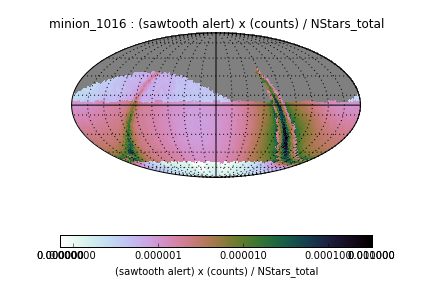
\includegraphics[width=5.25cm]{./figs/milkyway/galacticSN_SkyMap_Baseline.png}
  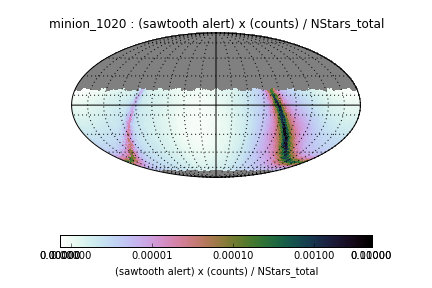
\includegraphics[width=5.25cm]{./figs/milkyway/galacticSN_SkyMap_PanSTARRS.png}
  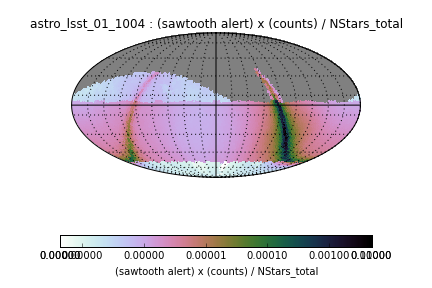
\includegraphics[width=5.25cm]{./figs/milkyway/galacticSN_SkyMap_PlaneWFD.png}
%  \includegraphics[width=6cm]{./figs/milkyway/galacticSN_Histogram_1092.pdf}
%  \includegraphics[width=6cm]{./figs/milkyway/galacticSN_Histogram_1189.pdf}
  \caption{Figure of merit $FoM_{preSN}$~describing LSST's sensitivity
  to any pre-Supernova outburst for the Galactic Supernova science case,
  broken down by sightline. $FoM_{preSN}$~is estimated for
  three OpSim runs (to-date); \opsimdbref{db:baseCadence} (left; Baseline
  cadence), \opsimdbref{db:opstwoPS} (center; PanSTARRS-like
  strategy), and {\tt astro\_lsst\_01\_1004} (which assigns Wide-Fast-Deep cadence to the inner Galactic Plane). The normalizing factors $N_{\ast, total}$ are $3.793 \times 10^{10}$~for both \opsimdbref{db:baseCadence} and {\tt astro\_lsst\_01\_1004} (that both strategies have the same $N_\ast$~is not a surprise since both cover the same area) and $3.692\times
  10^{10}$~for \opsimdbref{db:opstwoPS}. The imprint of reduced sampling towards
  the inner plane can be clearly seen for \opsimdbref{db:baseCadence}.
  Notice the difference in color scale between the panels. See \autoref{sec:MW_Disk:MW_Disk_analysis}}
\label{f_opSim_GalacticSN}
\end{center}
\end{figure}


% The Figures of Merit listed above must now be implemented and applied to the OpSim databases.

% The metrics listed above should be carefully compared between our proposed run and the baseline cadence.


% --------------------------------------------------------------------

\subsection{Discussion}
\label{sec:\secname:MW_Disk_discussion}

The Figures of Merit listed above must now be implemented within the
sims\_maf framework and applied to representative science cases.
See Table \ref{tab_SummaryMWDisk} at the end of this subsection for
initial efforts along these lines. We welcome input and volunteers for
this effort.

Qualitatively, however, we can note immediately that the current
baseline cadence (\opsimdbref{db:baseCadence}) partially excludes the
Galactic Plane from the deep-wide-fast survey and instead adopts a
nominal 30 visits per filter as part of a special proposal - which
also tends to cluster the visits in the inner Plane within the first
few years of the survey. This already seriously compromises the time
baseline (see \autoref{fig_astrom_ByTime_pmError} of
\autoref{sec:MW_Astrometry:MW_Astrometry_OpSim} for a demonstration applied to
proper motions).

%We have proposed an OpSim run that includes the Galactic Plane in the
%deep-wide-fast survey:

%\url{https://github.com/LSSTScienceCollaborations/ObservingStrategy/blob/master/opsim/Proposal_GP.md}

\begin{table}
  \begin{tabular}{l|p{6cm}|c|c|c|c|p{5cm}}
    FoM & Brief description & {\rotatebox{90}{\opsimdbref{db:baseCadence}}} & {\rotatebox{90}{\opsimdbref{db:opstwoPS}}} & {\rotatebox{90}{\scriptsize{\tt astro\_lsst\_01\_1004}  }} &  {\rotatebox{90}{future run 2}} & Notes \\
    \hline
    1.1 & \footnotesize{LMXB ellipsoidal variations}      & - & - & - & - & - \\
    1.2 & \footnotesize{Uncertainty in dwarf nova duty cycle}   & - & - & - & - &  \footnotesize{LSST as initial trigger} \\
    2.1 & \footnotesize{Fraction of Novae detected}       & - & - & - & - &  - \\
    2.2 & \footnotesize{Fraction of Nova alerts}       & - & - & - & - &  - \\
    3.1 & \footnotesize{Galactic Supernova pre-variability} & 0.13 & {\bf 0.83} & 0.73 & - & \footnotesize{Fraction of SN2010mc-like outbursts that LSST would detect; $FoM_{preSN} = f_{var} \times N_{\ast}$} \\
    4.1 & \footnotesize{Fraction of LSST-triggered microlens candidates} & - & - & - & - & - \\
    4.2 & \footnotesize{Uncertainty in derived planetary mass function} & - & - & - & - & \footnotesize{LSST as initial microlens trigger} \\
%    5.1a & \footnotesize{Median (over sight-lines) of the uncertainty in $E(B-V)$} & - & - & - & - & \footnotesize{(Most useful FoM probably a spatial map of the uncertainty.)} \\
%    5.1b & \footnotesize{Variance (over sight-lines) of the uncertainty in $E(B-V)$} & - & - & - & - & - \\
  \end{tabular}
\caption{Summary of figures-of-merit for the Galactic Disk science cases. The best value of each FoM is indicated in bold. Runs \opsimdbref{db:baseCadence} and \opsimdbref{db:opstwoPS} refer to the Baseline and PanSTARRS-like strategies, respectively. Column {\tt astro\_lsst\_01\_1004} refers to a recently-completed OpSim run that includes the Plane in Wide-Fast-Deep observations. See \autoref{sec:MW_Disk:MW_Disk_analysis}. }
\label{tab_SummaryMWDisk}
\end{table}


%Discussion: what risks have been identified? What suggestions could be
%made to improve this science project's figure of merit, and mitigate
%the identified risks?



% ====================================================================

\navigationbar
